\chapter{Implementation}
\label{chap:opendial}

\note{CHAPTER NOT READY YET!!}

This chapter exposes the most important features of the \opendial toolkit, which is a Java-based software toolkit developed to design and evaluate dialogue systems based on probabilistic rules. The toolkit implements all the data structures and algorithms detailed in this thesis.  It also served as a platform been used to carry out the experiments presented in Chapters \ref{chap:wozlearning}, \ref{chap:rllearning} and \ref{chap:user-evaluation}. 

\section{General architecture}

As already noted through this thesis, the dialogue system used in this thesis is integrated in a blackboard, event-driven architecture. The dialogue state corresponds to the blackboard upon which various system modules are attached.  The modules can both read and write to this dialogue state.  After each change, the dialogue state sends an event message to all its attached modules to inform them that the state has been updated. The modules can subsequently react to this update by generating new updates.  The process continues until the dialogue state stabilises.  

The \opendial toolkit allows system modules to run in parallel, using Java multi-threading. The possibility to execute modules in parallel is particularly important in dialogue architectures, as the system must be able to react to user input and contextual changes occurring at any time -- even while the system is still busy processing a previous update.  Many of the modules developed in the toolkit (such as planning and probabilistic inference) can also operate in anytime mode, which implies that they can be interrupted at any time and still provide an output. 

The current implementation of \opendial runs on a single platform.  Some specific modules can however remotely connect to external resources on the robotic platform to perform various tasks related to robot perception and motor control. Given the blackboard architecture of the toolkit, the framework could however be extended to support fully distributed systems in the future.

\subsection{System modules}

The system modules can be distinguished in to types: \begin{itemize}
\item Synchronous modules continuously monitor the dialogue state for relevant changes.  Their activation is thus in synchrony with the update events generated by the dialogue state.
\item Asynchronous modules operate independently of the dialogue state.  They typically relate to visual or speech perception tasks.
\end{itemize}

\note{turn-taking}

\note{agile-inspired methodology: frequent refactorings, implementation of JUnit test suites}

\subsubsection*{Speech recognition}

\subsubsection*{Natural language understanding}

\subsubsection*{Dialogue management}

\subsubsection*{Speech synthesis}

\subsubsection*{Robot perception}

\subsubsection*{Robot motion control}

\subsection{Graphical user interface}

The graphical user interface developed for the \opendial toolkit allows the system designer to monitor and control in real-time the current state of the system.  The interface is divided in two alternative views, shown as distinct tabs in the application window: the chat window and the dialogue state monitor.

\subsubsection*{Chat window}
The chat window presents the interaction history as a chat window.  The user inputs are shown as N-best lists together with their corresponding probabilities.  Figure \ref{fig:gui-chatbox} provides a screeenshot of the chat window. 

In addition to monitoring the interactions, the chat window can also be used to test the dialogue system by typing new user and system inputs in the input field at the bottom of the window.  The agent role can be switched in the drop-down field in the bottom right corner. 

\begin{figure}[h]
\centering
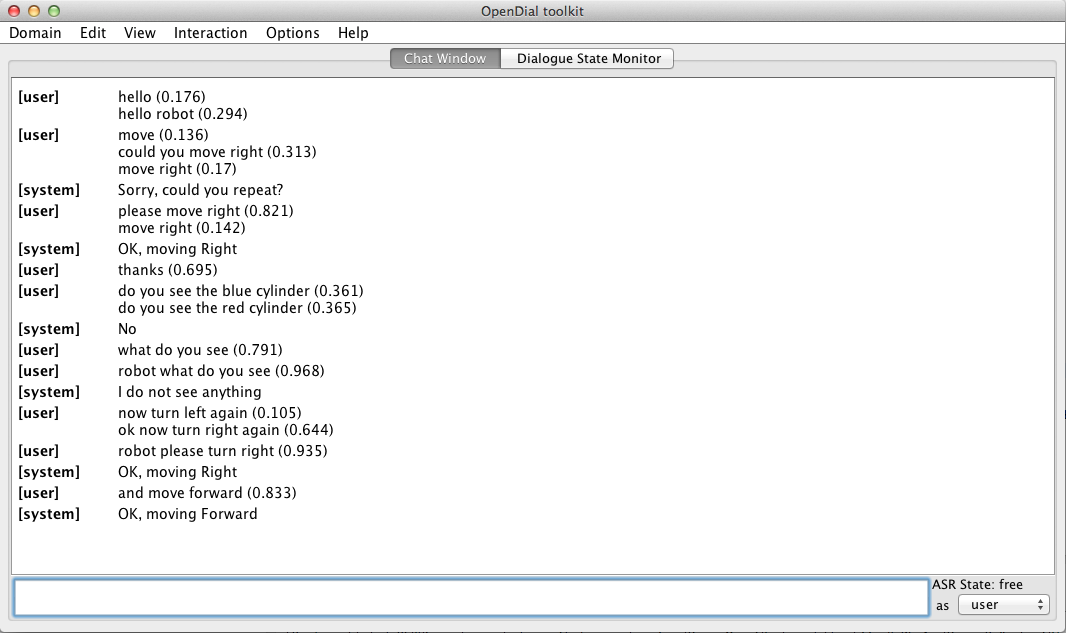
\includegraphics[scale=0.40]{imgs/gui-chatbox.png}
\caption{Graphical user interface showing the interaction history.}
\label{fig:gui-chatbox}
\end{figure}

\subsubsection*{Dialogue state monitor}

To allow the system designer to inspect the content of the dialogue state, a visualisation tool has also been integrated into \opendial .  The tool draws a graph with nodes corresponding to the state variables and directed edges corresponding to conditional dependencies.\footnote{The graphs are rendered using JUNG, which is a Java-based open source toolkit for drawing various kinds of graph structures -- cf. \begin{scriptsize}\url{http://jung.sourceforge.net}\end{scriptsize}.} An example of graph layout is shown in Figure \ref{fig:gui-bn}. The graph is dynamically refreshed after each update of the dialogue state. The graph layout is automatically calculated to optimise the visualisation. 

In addition to showing the current dialogue state, the dialogue state monitor can also record and store previous dialogue states.  The dialogue state to visualise can be selected among the list on the left side of the window. This functionality is useful to e.g. compare dialogue states with one another and analyse how the dialogue state is evolving over time. 

\begin{figure}[h] 
\begin{center}
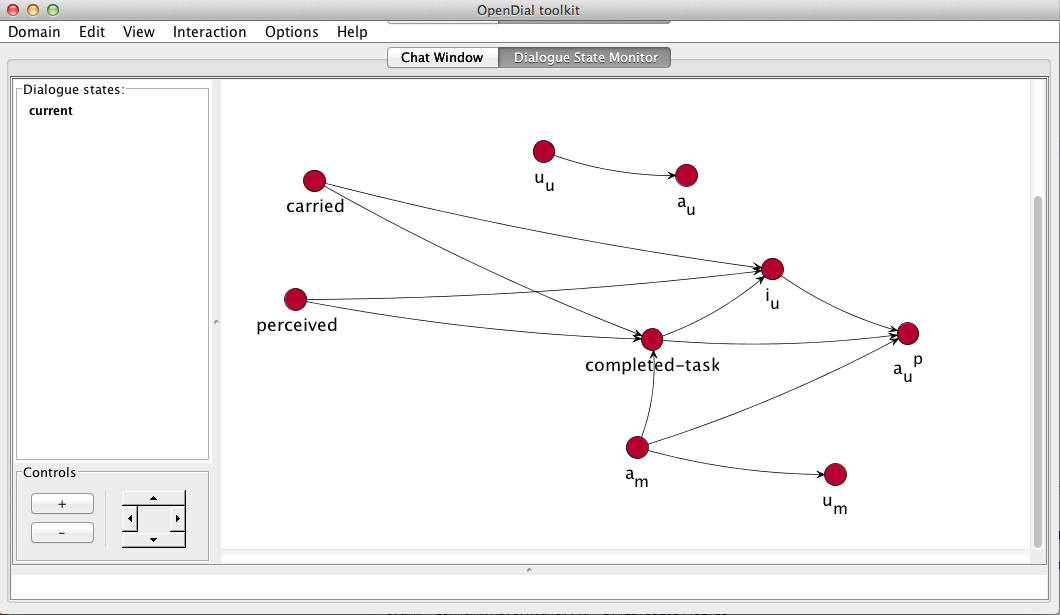
\includegraphics[scale=0.40]{imgs/gui-bn.png}
\end{center} 
\caption{Visualisation of the current dialogue state.}
\label{fig:gui-bn}
\end{figure}

The graph can be manipulated in multiple ways in order to e.g. inspect the content of specific state variables, add or remove evidence, or request the calculation of marginal distributions on selected set of variables.  The inference results are shown in the text area at the bottom of the window.  In addition, the system designer can also directly view the shape of selected probability distributions using the distribution viewer tool illustrated in Figure \ref{fig:gui-distribviewer}. Discrete probability distributions are shown as histograms, while continuous probability distributions are graphically represented by their probability density functions.\footnote{The graphical rendering of the probability distributions is done with the open source toolkit JFreeChart, cf. \begin{scriptsize}\url{http://jfreechart.sourceforge.net}\end{scriptsize}.} 


\begin{figure}[h] 
\begin{center}
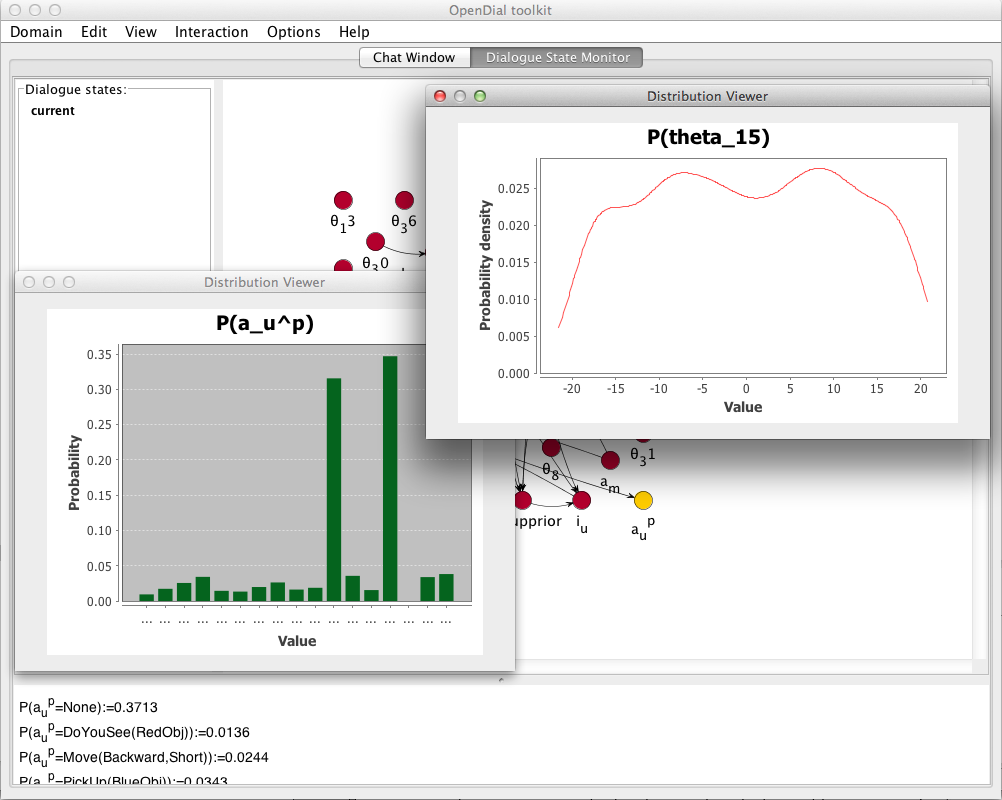
\includegraphics[scale=0.40]{imgs/gui-distribviewer.png}
\end{center} 
\caption{Distribution viewer showing both a discrete probability distribution for $P(a_u^p)$ and a continuous probability distribution $P(\theta_{15})$.}
\label{fig:gui-distribviewer}
\end{figure}

\section{Specification of dialogue domains}
\label{sec:domain-specification}

\subsection{Motivation}

Many reasoning tasks can be structured in terms of probabilistic rules.  Beyond the core probability and utility models for dialogue management, probabilistic rules have also been applied in our work to natural language understanding and generation tasks.  The dialogue domain designed for the user experiments in Chapter \ref{chap:user-evaluation} included for instance a total of 6 models: one dialogue act classification model, (triggered by the user utterance $u_u$), one action utility model (triggered by the user dialogue act $a_u$), three probability models to predict the effects of the system action on the context, the user intention and the next user action (all triggered by the system action $a_m$), and a generation model (triggered by the system action $a_m$).  The association of trigger variables to the rule-based models provides a simple and flexible a way to define the processing pipeline for the application.  Variables can function as triggers for more than one model, allowing models to be instantiated in parallel.


As argued in \cite{lison-semdial2012}, the expressive power of probabilistic rules allow them to capture the structure of many dialogue processing tasks.  Compared to traditional architectures in which the components are developed separately and rely on ad hoc representation formats, the use of a shared formalism to encode the domain models yields several advantages:
\begin{description}
\item [Transparency: ] The reliance on a common representation format provides a unified, transparent semantics for the dialogue state, since all state variables are described and related to one another through a principled framework grounded in probabilistic modelling.  This makes it possible to derive a semantic interpretation for the dialogue state as a whole -- in terms e.g. of a joint probability distribution over the state variables. 

\item [Domain portability: ]  As all domain-specific knowledge is declaratively specified in the rules, the system architecture is essentially reduced to a generic platform for rule instantiation and probabilistic inference.  This declarative design greatly enhances the system portability across domains, since adapting a system to a new domain only requires a rewrite or extension of the domain-specific rules, without having to reprogram a single component.  This stands in sharp contrast with ``black-box'' types of architectures where much of the task- and domain-specific knowledge is encoded in procedural form within the component workflow.

\item [Flexible workflow: ] Probability rules can design very flexible processing pipelines where state variables are allowed to depend or influence each other in any order and direction.  Models can be easily inserted or extended without requiring any change to the underlying platform. Furthermore, several models can be triggered concurrently on the same input/output variables.\footnote{Output distributions can indeed handle effect specifications arising from multiple, sometimes conflicting sources, as we have seen in Section \ref{sec:probruleinstantiation}.} This allows the system to take advantage of multiple, complementary modelling strategies while ensuring that the dialogue state remains consistent. 

\item [Joint optimisation: ] Finally, the use of a unified modelling formalism allows domain models to be optimised jointly instead of being tuned in isolation from one another. Joint optimisation has recently gained much attention in the dialogue system community to overcome the fragmentation of current system architectures and attempt to directly optimise the end-to-end conversational behaviour of the system \citep{Lemon:2011}. 

\end{description}

It should be noted that the architecture does not in any way preclude the integration of other types of processing modules in addition to rule-structured models, as long as these modules can read and update the dialogue state when relevant changes are detected. 


\subsection{Encoding format}

\note{general XML format, examples of rules}

\note{specification of parameters}


\section{Core algorithms}

\subsection{Inference}

\note{switching algorithm}

\subsection{Sampling techniques}

\subsection{Forward planning}


\note{switching algorithm, sampling methods for various distributions, kernel distributions}
\note{anytime behaviour}
\note{detail planning, state pruning}

\note{remarks on incrementality}

\section{Comparison with other architectures}

\note{Similarity to Olympus, Jaspis, Ariadne dialogue architectures?}

\section{Conclusion}
